% Figure 1 - Overview of the 2x2 factorial design (origin-and-levers / quadrant-cross).
% A fixed FT-UNetFormer baseline crossed over two binary levers:
%   horizontal axis = cross-dataset OpenEarthMap transfer (off -> on)
%   vertical   axis = class-balanced clsbal sampler        (off -> on)
% Baseline sits at the bottom-left origin; Full (shipped) at the top-right.
% The four cells share one plane split by a quadrant cross (not four separate boxes);
% on/off levers are marked with tick/cross; seed/tile/eval details live in the caption.
\documentclass[border=4pt]{standalone}
\usepackage[T1]{fontenc}
\usepackage{lmodern}
\usepackage{amsmath}
\usepackage{amssymb}
\usepackage{tikz}
\usetikzlibrary{positioning, arrows.meta, calc}

\newcommand{\offmark}{\textcolor{red!65!black}{$\boldsymbol{\times}$}}
\newcommand{\onmark}{\textcolor{green!45!black}{$\checkmark$}}

\begin{document}

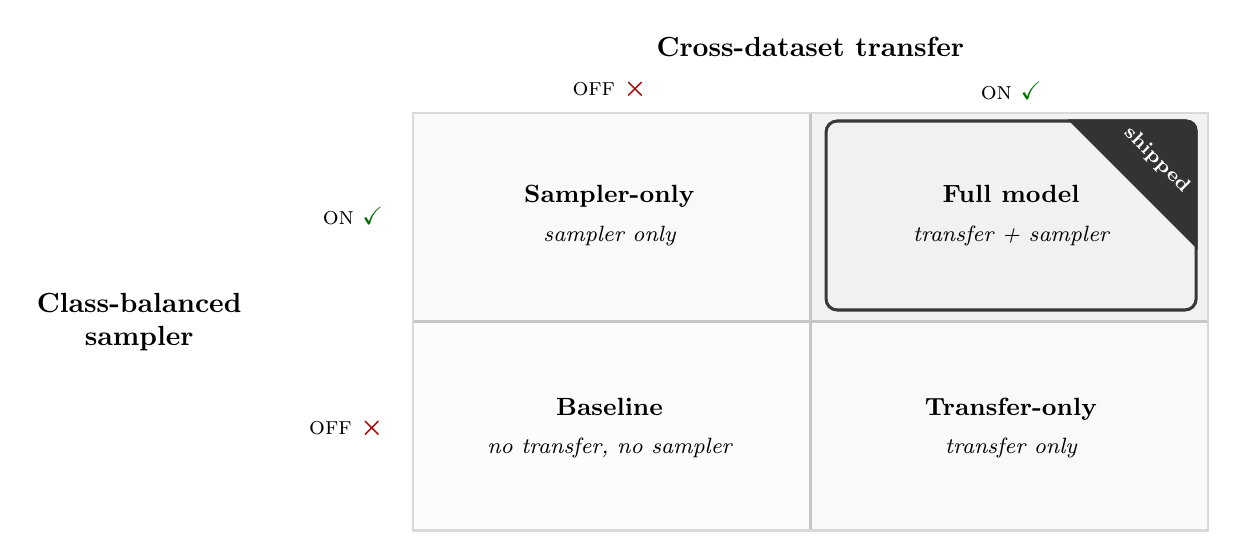
\begin{tikzpicture}[
  font=\small,
  >=Stealth,
  cell/.style={
    rounded corners=4pt,
    minimum width=4.7cm, minimum height=2.4cm,
    align=center, inner sep=6pt, draw=none,
    fill=none
  },
  full/.style={cell, line width=1.1pt, draw=black!78, fill=none},
  axislbl/.style={align=center, font=\bfseries},
  levelbl/.style={align=center, font=\small},
]

% ---- geometry (cell centres) ----
\def\cxl{-2.55}  % left  column centre (transfer OFF)
\def\cxr{2.55}   % right column centre (transfer ON)
\def\ryb{-2.7}   % bottom row centre   (sampler OFF)
\def\ryt{0}      % top    row centre   (sampler ON)

% extents for the quadrant cross
\def\xmin{-5.05}
\def\xmax{5.05}
\def\ymin{-4.0}
\def\ymax{1.3}
\def\xmid{0}
\def\ymid{-1.35}

% =====================================================
% BUILD-UP GRADIENT: quadrant tints, lightest at the baseline origin
% (bottom-left), darkest at Full (top-right). The two single-lever cells
% share one tint -- they are equidistant from the baseline.
% =====================================================
\fill[gray!2]  (\xmin,\ymin) rectangle (\xmid,\ymid); % baseline
\fill[gray!5]  (\xmid,\ymin) rectangle (\xmax,\ymid); % transfer-only
\fill[gray!5]  (\xmin,\ymid) rectangle (\xmid,\ymax); % sampler-only
\fill[gray!11] (\xmid,\ymid) rectangle (\xmax,\ymax); % full

% =====================================================
% QUADRANT CROSS (the two axes crossing the plane = the divider)
% =====================================================
\draw[gray!45, line width=1.0pt] (\xmin,\ymid) -- (\xmax,\ymid);
\draw[gray!45, line width=1.0pt] (\xmid,\ymin) -- (\xmid,\ymax);
% subtle frame around the plane
\draw[gray!30, line width=0.8pt] (\xmin,\ymin) rectangle (\xmax,\ymax);

% =====================================================
% FOUR FACTORIAL CELLS (quadrant intersections)
% =====================================================
\node[cell] (baseline) at (\cxl,\ryb) {%
  \textbf{Baseline}\\[3pt]
  {\footnotesize\itshape no transfer, no sampler}};

\node[cell] (transfer) at (\cxr,\ryb) {%
  \textbf{Transfer-only}\\[3pt]
  {\footnotesize\itshape transfer only}};

\node[cell] (sampler) at (\cxl,\ryt) {%
  \textbf{Sampler-only}\\[3pt]
  {\footnotesize\itshape sampler only}};

\node[full] (fullcell) at (\cxr,\ryt) {%
  \textbf{Full model}\\[3pt]
  {\footnotesize\itshape transfer + sampler}};

% shipped ribbon -- corner flag clipped to the rounded cell, clear of cell text
\begin{scope}
  \clip[rounded corners=4pt]
    ($(fullcell.south west)$) rectangle ($(fullcell.north east)$);
  \coordinate (tr) at (fullcell.north east);
  \fill[black!80]
    ($(tr)+(-1.7,0.05)$) -- ($(tr)+(0.05,0.05)$) -- ($(tr)+(0.05,-1.7)$) -- cycle;
\end{scope}
\node[white, font=\scriptsize\bfseries, rotate=-45, anchor=center]
  at ($(fullcell.north east)+(-0.52,-0.52)$) {shipped};

% =====================================================
% COLUMN (TRANSFER) HEADERS -- horizontal, short
% =====================================================
\node[axislbl, anchor=south] at (\xmid,\ymax+0.6) {Cross-dataset transfer};
\node[levelbl, anchor=south] at (\cxl,\ymax+0.05) {{\sc off}~\offmark};
\node[levelbl, anchor=south] at (\cxr,\ymax+0.05) {{\sc on}~\onmark};

% =====================================================
% ROW (SAMPLER) HEADERS -- horizontal, short
% =====================================================
\node[axislbl, align=center, anchor=east] at (\xmin-2.05,\ymid)
  {Class-balanced\\sampler};
\node[levelbl, anchor=east] at (\xmin-0.25,\ryb) {{\sc off}~\offmark};
\node[levelbl, anchor=east] at (\xmin-0.25,\ryt) {{\sc on}~\onmark};

\end{tikzpicture}

\end{document}
